\documentclass[conference]{IEEEtran}
\IEEEoverridecommandlockouts
% The preceding line is only needed to identify funding in the first footnote. If that is unneeded, please comment it out.
\usepackage{cite}
\usepackage{amsmath,amssymb,amsfonts}
\usepackage{algorithmic}
\usepackage{graphicx}
\usepackage{textcomp}
\usepackage{xcolor}
\usepackage{hyperref}

\def\BibTeX{{\rm B\kern-.05em{\sc i\kern-.025em b}\kern-.08em
    T\kern-.1667em\lower.7ex\hbox{E}\kern-.125emX}}
\begin{document}

\title{Gomoku Champion: A Reinforcement Learning Model to Play \textit{Five in a Row}\\
{}
\thanks{}
}

\author{\IEEEauthorblockN{Bruce Jianye Liu}
\IEEEauthorblockA{\textit{Stanford University SCPD}\\
Waterloo, Ontario, Canada \\
bruceliu@stanford.edu}
\and
\IEEEauthorblockN{David Douglas Wickland}
\IEEEauthorblockA{\textit{Stanford University SCPD}\\
Guelph, Ontario, Canada \\
wickland@stanford.edu}
}

\maketitle

\begin{IEEEkeywords}
Gomoku, reinforcement learning, deep neural network, artificial intelligence
\end{IEEEkeywords}

\section{Problem Statement and Task Definition}
 In our paper, we propose a reinforcement learning model which learns to play the classic Japanese chess game Gomoku, also called \textit{Five in a Row}. Gomoku is an abstract strategy board game with two players taking turns to place a stone of their color on an empty grid. The first player to connect five adjacent stones horizontally, vertically, or diagonally wins. If no player connects 5 adjacent stones, the game is a draw. Figure \ref{gomoku-near-win} and Figure \ref{gomoku-win} illustrate a board state for a near-win scenario and a win scenario respectively.
 
 \begin{figure}[h]
    \centering
    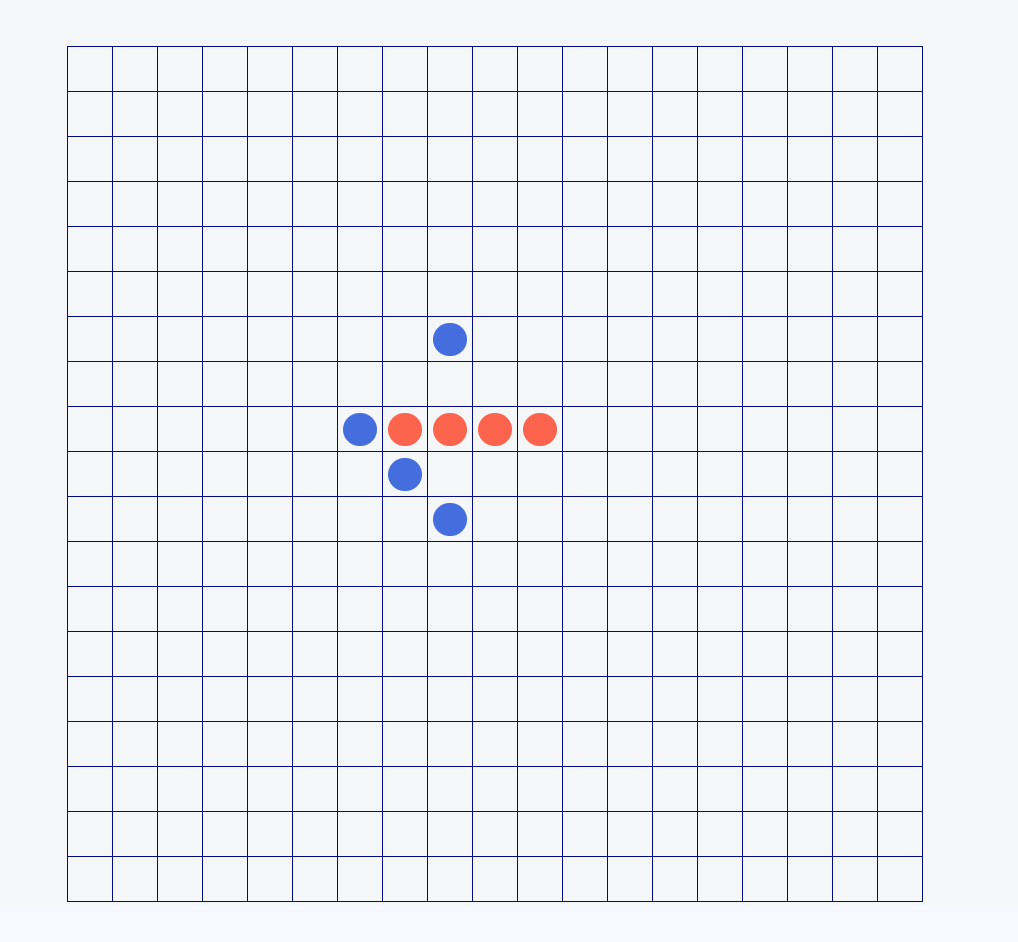
\includegraphics[width=0.25\textwidth]{images/gomoku-nearwin.png}
    \caption{A near-win for red}
    \label{gomoku-near-win}
\end{figure}

\begin{figure}[h]
    \centering
    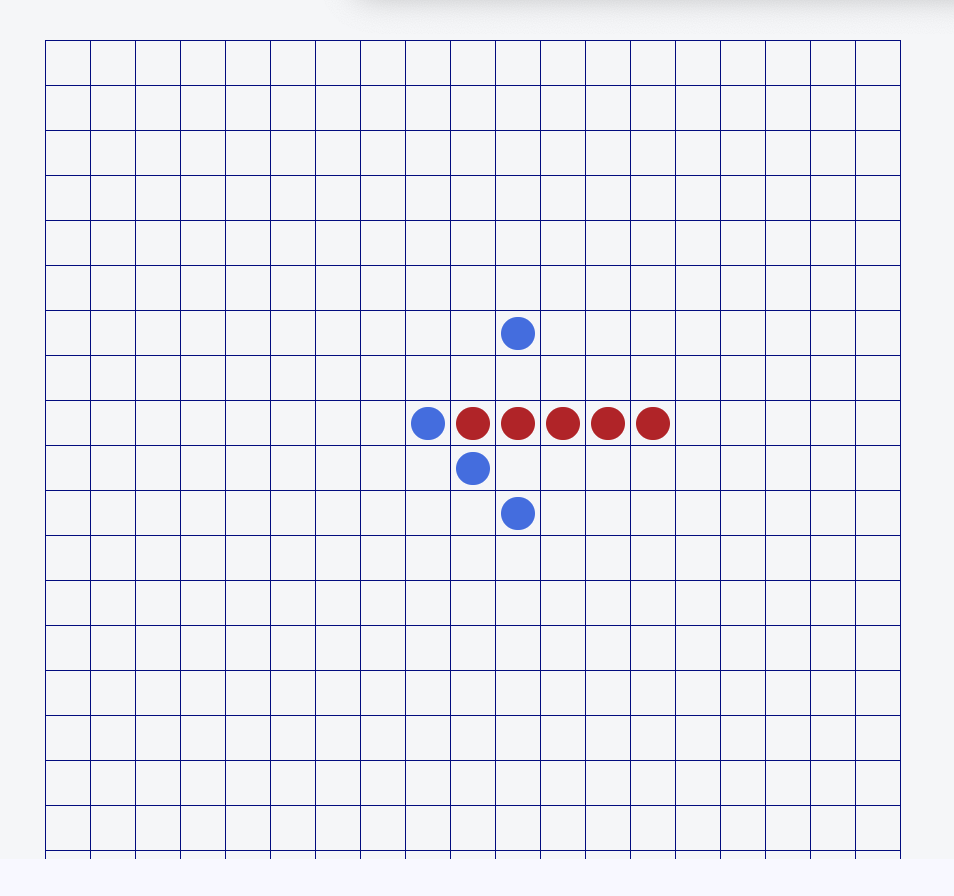
\includegraphics[width=0.25\textwidth]{images/gomoku-win.png}
    \caption{A win for red}
    \label{gomoku-win}
\end{figure}
 
 To win the game, it requires players to learn planning, strategy, and tactics. Gomoku is a simplified version of the game Go. Having a smaller search space enables us to apply the knowledge in CS221 in practice with limited time and resources. The model acts like a human player and attempts to win against its opponent.

\section{Model Input/Output}
The model input is an $n$ x $n$ matrix $M$, representing the current state of the playing board. Each coordinate $c$ in $M$ can be occupied by the opponent, occupied by the player, or unoccupied $s.t. \text{ }c \in \{-1, 0, 1 \}$. For a coordinate $c$ of location $(x, y)$ in matrix $M$, the possible states $S$ can be:

\[
    c(x, y) =
\begin{cases}
    -1 & \text{if occupied by opponent}\\
    1  &\text{if occupied by player}\\
    0  & \text{otherwise (unoccupied)}
\end{cases}
\]

If there are unoccupied squares on the board, the output of the model will be a coordinate of the horizontal and vertical location of the next piece the model will place (e.g. $(5, 7)$). If there are no unoccupied squares, the game concludes in a draw.

\section{An Evaluation Metric}
Mnih et al. demonstrated that the total reward the agent collects in each episode tends to be very noisy, and vary a lot during training; whereas action value $Q$ looks more stable during the training \cite{b1}. If the average $Q$ value increases smoothly in the training, it means our model is improving and learning stably.

Reward and Score Comparison with a random policy, SARSA, and an expert player, will allow us to evaluate how our model is performing. SARSA will be beneficial since it is an on-policy learning algorithm that can learn the value of the policy being carried out, as well as the exploration steps.

We will construct a dataset by scraping game actions and states from \href{https://gomokuonline.com}{Gomoku Online} and use this dataset as replay memory for future training.

\subsection{Experience Replay}
Each round of playing, we will record the history as $e$ that contains a series of state, action, and reward
$$e = [s_0, a_0, r_1, s_1, a_1, r_2, ...]$$

Playing $t$ round gives us a set of training data
$$E = \{e_1, e_2, e_3, ..., e_t\}$$

\subsection{Play Against Itself}
We intend to duplicate the model into two competing models $A$ and $B$, that will play against each other. The models will alternate placing a stone on the board until the game concludes in a win or a draw. At the end, if the game outcome is a win, the model that won will receive a positive reward and model that lost will receive a negative reward. If a game outcome is a draw, both models will receive a zero reward.

\subsection{Play Against Classic Engine}
We will use a classic game engine with hard-coded rules to assist the model in learning the basic rules of the game.

\section{Related Works}\label{AA}
The Atari game paper by Mnih et al. and the AlphaGo paper by Silver et al. were milestones in field of adversarial game reinforcement learning \cite{b1, b2}. Their models could out-perform human experts, laying the foundation of reinforcement learning in game modeling. More recently Zheng, Fu and Yu modified the AlphaGo model to use curriculum learning applied to game Gomoku \cite{b3}. Wang and Huang also created a Gomoku solver with deep learning and genetic algorithms \cite{b5}. Dongbin, Zhang, Dai proposed a deep network model by self-teaching Adaptive Dynamic Programming \cite{b6}.

\section{Baseline and Oracle}
Our baseline will be to compete against a model with a random action policy. The oracle we have selected will be the win over a average human players. If the model can win 10 consecutive games against an average human player, we will consider this as a relatively strong performance.

\section{Methodology}
We will be using a simulated environment by integrating our model with \href{https://gomokuonline.com}{Gomoku Online}. As well, we will create our own simulated environment in order to allow our model to play itself. There are several examples of Gomoku implemented online which we can leverage to design and implement our simulated environment.

The Gomoku chess game can be modeled as a Markov Problem, where we could build a deep neural policy $\pi$ to predict its next piece location $(x, y)$ which meets $\pi(s) = a$. The environment generates its reward and next state $s^\prime$ of the board.

We have instead chosen to train our model using reinforcement learning, since the search space is too large to be tractable when modeled as a Markov Decision Process (MDP) using an exhaustive search (e.g. Uniform Cost Search).

\section{Description of the challenges}
One challenge will be to identify a suitable reward function and discount that will train our model to be competitive in an adversarial paradigm. We need to develop a model that can win swiftly, as this is essential behaviour when competing. Another challenge will be to teach our model how to act optimally at the edges of the playing board. These states are rarely encountered in typical games, but will alter the optimal policy once the center of the board is mostly occupied.

Alpha-beta pruning may be a useful tool in guiding our model to make better decisions since it is an adversarial search algorithm that has been successfully applied to many two-player games \cite{b4}.

\begin{thebibliography}{00}
\bibitem{b1} Mnih, Volodymyr, et al. "Playing atari with deep reinforcement learning." arXiv preprint arXiv:1312.5602 (2013).
\bibitem{b2}Silver, David, et al. "Mastering the game of Go with deep neural networks and tree search." nature 529.7587 (2016): 484-489.
\bibitem{b3}Xie, Zheng, XingYu Fu, and JinYuan Yu. "AlphaGomoku: An AlphaGo-based Gomoku Artificial Intelligence using Curriculum Learning." arXiv preprint arXiv:1809.10595 (2018).
\bibitem{b4} C.T. Kuo. Jonathan Artificial Intelligence at play - connect Four (Minimax algorithm explained), Medium, Analytics Vidhya, 2021, May. \href{https://medium.com/analytics-vidhya/artificial-intelligence-at-play-connect-four-minimax-algorithm-explained-3b5fc32e4a4f}{\textit{link-to-article}}
\bibitem{b5}Wang, Junru, and Lan Huang. "Evolving Gomoku solver by genetic algorithm." 2014 IEEE Workshop on Advanced Research and Technology in Industry Applications (WARTIA). IEEE, 2014.
\bibitem{b6}Zhao, Dongbin, Zhen Zhang, and Yujie Dai. "Self-teaching adaptive dynamic programming for Gomoku." Neurocomputing 78.1 (2012): 23-29.

\end{thebibliography}

\end{document}
